\documentclass[12pt,compress,aspectratio=169,dvipsnames]{beamer}
\input{../../mybeamer}
\usepackage{mathtools}
  
\title{Class 2A: Advanced Graphing Techniques}
\subtitle{AP Physics C--Mechanics}
\input{../../me}
\input{../../mycommands}

\begin{document}

\begin{frame}
  \titlepage
\end{frame}



\begin{frame}{Advanced Graphing Technique: $x$ vs.\ $t^2$}
  \begin{columns}[T]
    \column{.4\textwidth}
    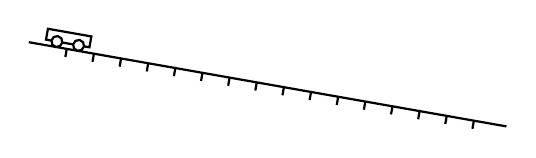
\begin{tikzpicture}[scale=.7,rotate around={-10:(9,0)}]
      \draw[thick] (0,0)--+(8.8,0);
      \draw[thick] (.3,.1) rectangle +(.8,.2);
      \draw[thick,fill=black!2] (.5,.1) circle (.1);
      \draw[thick,fill=black!2] (.9,.1) circle (.1);
      \foreach \x in {.7,1.2,...,8.5}
      \draw[thick](\x,0)--+(0,-.15); % node[below]{\tiny$\x$};
    \end{tikzpicture}

    \column{.6\textwidth}
    A toy cart rolls down a ramp from rest (i.e.\ $v_0=0$). At regular
    distances, time is recorded. In this case, the acceleration of the cart
    \emph{should} be constant. Can we determine the car's acceleration?
  \end{columns}
  
  \vspace{.3in}
  \begin{columns}[T]
    \column{.51\textwidth}
    \uncover<2->{\color{magenta}
      
      \vspace{.03in}Based on the data, we can plot an $x$--$t$ graph.
      Unfortunately this graph would not be very helpful in determining
      acceleration.

      \begin{tabular}{c|c}
        $x$ & $t$ \\\hline
        $x_0$ & 0 \\
        $x_1$ & $t_1$\\
        \vdots & \vdots \\
        $x_N$ & $t_N$
      \end{tabular}
      \hspace{.2in}
      \begin{minipage}{.4\textwidth}
        \begin{tikzpicture}
          \draw[axes](0,0)--(0,2) node[right]{$x$};
          \draw[axes](0,0)--(2,0) node[right]{$t$};
          \draw[smooth,domain={0:1.8},very thick] plot(\x,{.4*\x*\x+.3});
        \end{tikzpicture}
      \end{minipage}
    }

    \column{.49\textwidth}
    \uncover<3>{\color{violet}
      If, instead, we plot $x$--$t^2$, the graph would be \emph{linear}, and
      the slope will tell us about the acceleration.

      \begin{tabular}{c|c}
        $x$ & $t^2$ \\\hline
        $x_0$ & 0 \\
        $x_1$ & $t_1^2$\\
        \vdots & \vdots \\
        $x_N$ & $t_N^2$
      \end{tabular}
      \hspace{.2in}
      \begin{minipage}{.4\textwidth}
        \begin{tikzpicture}
          \draw[axes] (0,0)--(0,2) node[right]{$x$};
          \draw[axes] (0,0)--(2,0) node[right]{$t^2$};
          \draw[very thick] (0,.3)--(1.8,1.8);
        \end{tikzpicture}
      \end{minipage}
    }
  \end{columns}
\end{frame}



\begin{frame}{Advanced Graphing Technique: $x$ vs.\ $t^2$}
  When we plot $x$ as a function of $t^2$ instead of a function of $t$, we are
  essentially doing this to the kinematic equation (from a few slide ago):

  \eq{-.1in}{
    \underbracket[1pt]{x}_y=\underbracket[1pt]{x_0}_b +
    \underbracket[1pt]{\frac12a}_m\underbracket[1pt]{t^2}_x
  }
  
  \vspace{-.05in}and turning it into a linear function in the form $y=mx+b$
  that is familiar to everyone.
  \begin{itemize}
  \item The slope of the $x$ vs. $t^2$ graph is $\dfrac12a$ (or acceleration
    is 2 times the slope)
  \item If the $x$ vs.\ $t^2$ graph is \emph{not} linear, we will know that
    our assumption of constant acceleration was incorrect, and that there are
    other factors that we neglected
  \end{itemize}
\end{frame}


\begin{frame}{Advanced Graphing Technique: $v^2$ vs.\ $\Delta x$}
  \begin{columns}[T]
    \column{.4\textwidth}
    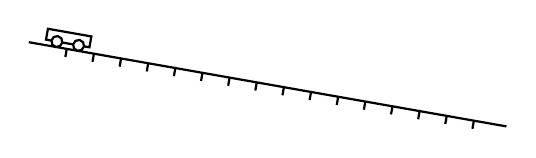
\begin{tikzpicture}[scale=.7,rotate around={-10:(9,0)}]
      \draw[thick] (0,0)--+(8.8,0);
      \draw[thick] (.3,.1) rectangle +(.8,.2);
      \draw[thick,fill=black!2] (.5,.1) circle (.1);
      \draw[thick,fill=black!2] (.9,.1) circle (.1);
      \foreach \x in {.7,1.2,...,8.5}
      \draw[thick](\x,0)--+(0,-.15); % node[below]{\tiny$\x$};
    \end{tikzpicture}

    \column{.6\textwidth}
    A toy cart rolls down a ramp. At regular positions $x$ along the ramp, the
    cart's velocity $v$ is recorded instead. Again, acceleration \emph{should}
    be constant. Can we determine the car's acceleration from the data?
  \end{columns}

  \vspace{.3in}
  \begin{columns}[T]
    \column{.5\textwidth}
    \uncover<2->{\color{magenta}
      
      \vspace{.03in}Plotting the data would give us a $v$--$x$ graph.
      Unfortunately (again) this graph would not help us find the acceleration.

      \begin{tabular}{c|c}
        $x$ & $v$ \\\hline
        $x_0$ & $v_0$ \\
        $x_1$ & $v_1$\\
        \vdots & \vdots \\
        $x_N$ & $v_N$
      \end{tabular}
      \hspace{.2in}
      \begin{minipage}{.6\textwidth}
        \begin{tikzpicture}
          \draw[axes] (0,0)--(0,2) node[right]{$v$};
          \draw[axes] (0,0)--(2,0) node[right]{$x$};
          \draw[smooth,domain={0:1.8},samples=40,very thick]
          plot(\x,{\x^.5+.3});
        \end{tikzpicture}
      \end{minipage}
    }

    \column{.5\textwidth}
    \uncover<3>{\color{violet}
      But if we plot $v^2$ vs.\ $\Delta x$, the graph would be \emph{linear},
      and the slope will give us information about acceleration.

      \begin{tabular}{c|c}
        $v^2$ & $\Delta x$ \\\hline
        $v_0$ & 0 \\
        $v_1$ & $x_1-x_0$\\
        \vdots & \vdots \\
        $v_N$ & $x_N-x_0$
      \end{tabular}
      \hspace{.2in}
      \begin{minipage}{.4\textwidth}
        \begin{tikzpicture}
          \draw[axes] (0,0)--(0,2) node[right]{$v^2$};
          \draw[axes] (0,0)--(2,0) node[right]{$\Delta x$};
          \draw[very thick] (0,.3)--(1.8,1.8);
        \end{tikzpicture}
      \end{minipage}
    }
  \end{columns}
\end{frame}



\begin{frame}{Velocity Squared vs.\ Displacement}
  If velocity and position are given, then the relationship would be best
  expressed using this kinematic equation (we have studied a few slide ago):

  \eq{-.1in}{
    \underbracket[1pt]{v^2}_y=\underbracket[1pt]{v_0^2}_b+
    \underbracket[1pt]{2a}_m
    \underbracket[1pt]{(x-x_0)}_x
  }

  by plotting $v^2$ vs. $\Delta x=x-x_0$, we again have a linear function in the
  form of $y=mx+b$.
  \begin{itemize}
  \item The slope of the graph is two times the acceleration $m=2a$ (i.e.\
    acceleration is one half of the slope).
  \item The square of the initial velocity ($v_0^2$) is the $y$-intercept
  \item \emph{If} our assumption was incorrect (i.e.\ acceleration is \emph{not}
    constant) then the line would not be straight
  \end{itemize}
\end{frame}



\begin{frame}{Graphing ``Linear'' Functions: Example}
  This concept extends to graphing other physical relationships not related to
  kinematics. For example, to find the index of refraction of a material using
  Snell's law, we can plot $\sin\theta_1$ vs.\ $\sin\theta_2$ (instead than
  $\theta_1$ vs.\ $\theta_2$). The slope is the ratio of the indices $n_1/n_2$:

  \eq{-.1in}{
    \underbracket[1pt]{\sin\theta_2}_y=
    \underbracket[1pt]{\left[\frac{n_1}{n_2}\right]}_m
    \underbracket[1pt]{\sin\theta_1}_x
  }

  In an experiment, we can vary the incident angle $\theta_1$ in a medium with
  a known index ($n_1$), and measure the corresponding refracted angle
  $\theta_2$. Once the slope of the graph ($n_1/n_2$) is known, we can find
  $n_2$.
\end{frame}



\begin{frame}{Graphing ``Linear'' Functions: Another Example}
  To relate the period of oscillation (the time it takes to swing back and
  forth once) of a simple pendulum to the length of the pendulum, plot $T$
  vs.\ $\sqrt\ell$:

  \eq{-.15in}{
    \underbracket[1pt]{T}_y=\underbracket[1pt]{\frac{2\pi}{\sqrt g}}_m
    \underbracket[1pt]{\sqrt\ell}_x
  }

  or alternatively, by squaring both sides of the equation to relate $T^2$ to
  $\ell$:

  \eq{-.15in}{
    \underbracket[1pt]{T^2}_y=\underbracket[1pt]{\left[\frac{4\pi^2}g\right]}_m
    \underbracket[1pt]{\ell}_x
  }

  We can change the length of the pendulum $\ell$ and measure the period $T$ of
  the oscillation.
\end{frame}
\end{document}
